% fsm_diagram.tex -- State transition diagram for the Cache Controller FSM
% Owner: Member 2 (Controller FSM & Tag Comparator)
% Compiles standalone to PDF; include in the IEEE report with:
%   \includegraphics[width=\columnwidth]{figures/fsm_diagram.pdf}

\documentclass[tikz,border=8pt]{standalone}
\usetikzlibrary{arrows.meta,calc,positioning}

\begin{document}
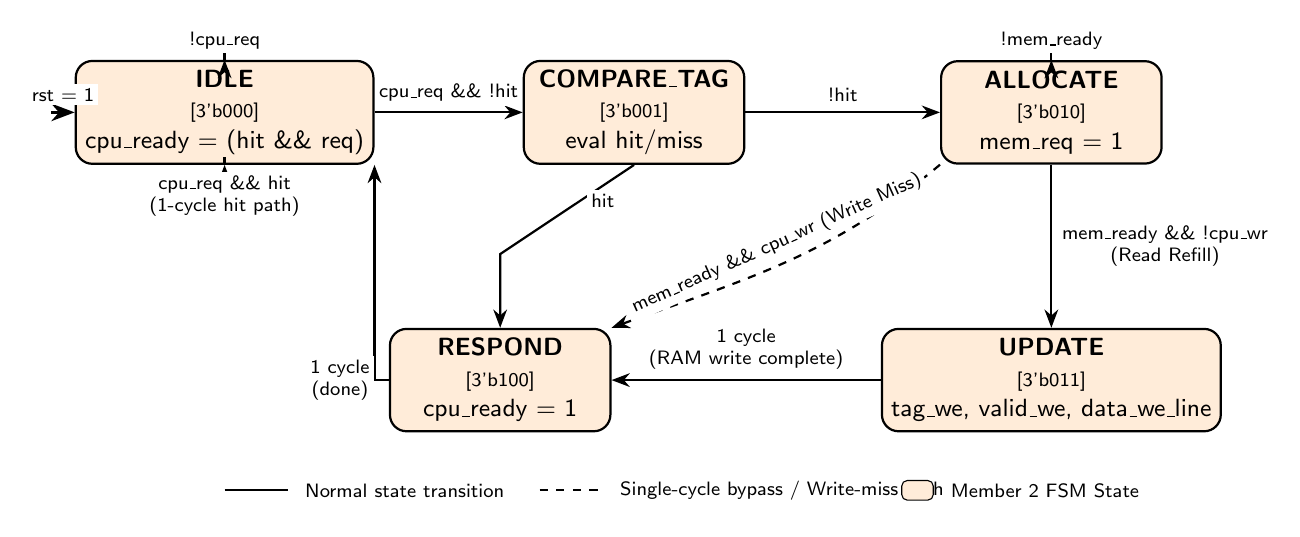
\begin{tikzpicture}[
    >=Stealth, font=\sffamily\small,
    state/.style={draw, thick, rounded corners=6pt, align=center,
                 minimum height=1.3cm, minimum width=2.8cm, fill=orange!15},
    lbl/.style={font=\sffamily\scriptsize, fill=white, inner sep=1.5pt, align=center},
    action/.style={font=\sffamily\tiny\bfseries, text=blue!80!black}
]

% ---------------- State Nodes ----------------
\node[state] (idle) at (0, 0) {
    \textbf{IDLE} \\ \scriptsize [3'b000] \\
    \action{cpu\_ready = (hit \&\& req)}
};

\node[state] (compare) at (5.2, 0) {
    \textbf{COMPARE\_TAG} \\ \scriptsize [3'b001] \\
    \action{eval hit/miss}
};

\node[state] (allocate) at (10.5, 0) {
    \textbf{ALLOCATE} \\ \scriptsize [3'b010] \\
    \action{mem\_req = 1}
};

\node[state] (update) at (10.5, -3.4) {
    \textbf{UPDATE} \\ \scriptsize [3'b011] \\
    \action{tag\_we, valid\_we, data\_we\_line}
};

\node[state] (respond) at (3.5, -3.4) {
    \textbf{RESPOND} \\ \scriptsize [3'b100] \\
    \action{cpu\_ready = 1}
};

% ---------------- Reset Vector ----------------
\draw[->, very thick] (-2.2, 0) -- node[lbl, above=2pt]{rst = 1} (idle.west);

% ---------------- Transitions ----------------
% 1. IDLE self-loop
\draw[->, thick] (idle.north) to [out=115, in=65, looseness=4]
    node[lbl, above=2pt]{!cpu\_req} (idle.north);

% 2. Fast-path Read/Write Hit loop on IDLE
\draw[->, thick, dashed] (idle.south) to [out=245, in=295, looseness=4]
    node[lbl, below=2pt]{cpu\_req \&\& hit\\(1-cycle hit path)} (idle.south);

% 3. IDLE -> COMPARE_TAG on miss
\draw[->, thick] (idle.east) --
    node[lbl, above=2pt]{cpu\_req \&\& !hit} (compare.west);

% 4. COMPARE_TAG -> ALLOCATE on miss
\draw[->, thick] (compare.east) --
    node[lbl, above=2pt]{!hit} (allocate.west);

% 5. COMPARE_TAG -> RESPOND on hit (multi-cycle request)
\draw[->, thick] (compare.south) --
    node[lbl, right=2pt, pos=0.4]{hit} (3.5, -1.8) -- (respond.north);

% 6. ALLOCATE self-loop (waiting for memory latency)
\draw[->, thick] (allocate.north) to [out=115, in=65, looseness=4]
    node[lbl, above=2pt]{!mem\_ready} (allocate.north);

% 7. ALLOCATE -> UPDATE on read miss refill ready
\draw[->, thick] (allocate.south) --
    node[lbl, right=2pt]{mem\_ready \&\& !cpu\_wr\\(Read Refill)} (update.north);

% 8. ALLOCATE -> RESPOND on write miss (no-write-allocate, skips UPDATE)
\draw[->, thick, dashed] (allocate.south west) to [out=220, in=20]
    node[lbl, above=2pt, sloped]{mem\_ready \&\& cpu\_wr (Write Miss)} (respond.north east);

% 9. UPDATE -> RESPOND
\draw[->, thick] (update.west) --
    node[lbl, above=2pt]{1 cycle\\(RAM write complete)} (respond.east);

% 10. RESPOND -> IDLE
\draw[->, thick] (respond.west) -|
    node[lbl, pos=0.3, left=2pt]{1 cycle\\(done)} (idle.south east);

% ---------------- Legend ----------------
\begin{scope}[shift={(0, -4.8)}]
    \draw[thick] (0, 0) -- (0.8, 0);
    \node[anchor=west, font=\sffamily\scriptsize] at (0.9, 0) {Normal state transition};
    \draw[thick, dashed] (4.0, 0) -- (4.8, 0);
    \node[anchor=west, font=\sffamily\scriptsize] at (4.9, 0) {Single-cycle bypass / Write-miss path};
    \node[draw, fill=orange!15, rounded corners=2pt, minimum width=0.4cm, minimum height=0.25cm] at (8.8, 0) {};
    \node[anchor=west, font=\sffamily\scriptsize] at (9.1, 0) {Member 2 FSM State};
\end{scope}

\end{tikzpicture}
\end{document}
